\chaptertitle{Introduction}
\label{chap:intro}
\introformatting

\lettrine{I}{nternet} est, à de nombreux égards, l'une des plus stupéfiantes
constructions humaines. Ce réseau né à la fin des années 60 pour relier entre
elles quelques unités logiques constitue aujourd'hui un gigantesque maillage,
sans centre clairement identifié, qui permet des communications très rapides
entre des centaines de millions de terminaux\cite{consotium2010isc}. Plus qu'un
réseau de télécommunication, Internet s'impose aujourd'hui comme {\em le} réseau
unifié, qui sert de base à d'innombrables édifices applicatifs. Des couriers
électroniques à la vidéophonie en passant par les jeux, les transactions
bancaires et les encyclopédies en lignes, toutes ces fonctionalités avancées
reposent, au dessus d'un empilement de couches d'abstraction, sur le réseau
Internet. Pour fonctionner, elles délèguent la problématique de l'acheminement
de l'information à Internet.

Cette confiance dans la robustesse et la fiabilité du réseau est justifiée par
son histoire. Internet n'a jamais été ``éteint'', ni même sévèrement menacé dans
son fonctionnement. Si des pannes ont temporairement perturbé son
fonctionnement, cela n'est arrivé que ponctuellement et dans une mesure toute
relative. Paradoxalement, pourtant, Internet n'a pas été imaginé et fabriqué
pour être capable de desservir des milliards d'utilisateurs, qui chaque jour à
travers le réseau envoient des centaines de milliards de courriers
électroniques, visionnent des milliards de vidéos, effectuent des dizaines de
millions d'appels en téléphonie Internet, des milliards de recherches, sur plus
d'un milliard de sites web et pour un traffic qui totalise plusieurs milliards
de GB de données\cite{internetlivestats}. En revanche, l'histoire a révélé que
sa nature décentralisée permet une très grande souplesse et une très grande
robustesse, ce qui a donc permis à de nombreux acteurs publics et industriels de
participer à son développement avec relativement peu de gouvernance. De telle
sorte que de très nombreux acteurs ont pu connecter leur réseau sur Internet,
l'agrandissant du même coup, en y rajoutant leurs propre briques, parfois
incompatibles avec les autres, mais sans remettre en cause l'intégrité d'un
réseau intrinsèquement très robuste. Internet est, aujourd'hui, le résultat de
son histoire riche et complexe, plutôt qu'un produit imaginé et conçu par une
entité clairement définie et traçable.

Pour cette raison, s'il est indiscutable qu'Internet ``fonctionne'', il n'existe
nulle part de carte complète du réseau. Certaines des propriétés les plus
élémentaires de la structure du réseau Internet, qu'on appelle aussi la {\em
topologie d'Internet}, telles que sa taille totale, la quantité d'information
réelle qui y circule, ou même sa forme générale, sont aujourd'hui inconnues ou
au mieux incertaines et parfois contestées. Il est donc très difficile de
raisonner ou de modéliser Internet dans sa globalité. Nous n'avons qu'une
connaissance très empirique du socle fondamental d'une quantité toujours
croissante de nos activités qui échappe assez largement à l'analyse.
Une meilleure connaissance du réseau est essentielle à la fois pour pouvoir
confirmer des acquis empiriques, en particulier concernant la fiabilité du
réseau à l'égard des pannes, mais aussi pour rechercher des optimisations,
notamment du routage, ou pour identifier des faiblesses, par exemple face à une
attaque ciblée, physique ou logicielle. Plusieurs approches ont été explorées
pour obtenir une connaissance plus approfondie de la topologie d'Internet, mais
se sont heurtées à de nombreux obstacles à la fois théoriques et pratiques, et
ont conduit à des résultats mitigés.

Cette thèse se positionne dans ce contexte, l'objectif central étant de
développer une méthode de mesure fiable pour évaluer certaines des propriétés
les plus importantes de la topologie d'Internet.
Nous prendrons le soin de présenter précisément l'importance, la structure, et
l'historique de nos objets d'intérêt, puisque la topologie d'Internet peut
s'interpréter à différents niveaux d'abstraction que nous décrirons. Nous
présenterons les approches historiques, leurs résultats et leurs limites, avant
de présenter notre propre approche. Nous terminerons ce chapitre introductif par
une présentation de l'organisation de cette thèse.

\newpage

\section{Préliminaires}

Une partie de la difficulté des travaux autours de la topologie d'Internet
repose sur la relation complexe entre les différents éléments du réseau, leur
rôle exact, et la manière dont ils sont modélisés. Le modèle que l'on choisit de
considérer dépend bien sûr de la nature du problème que l'on souhaite étudier et
plusieurs modèles peuvent revendiquer le nom de ``topologie d'Internet''. Cette
imprécision dans les définitions des objets étudiés est une source historique de
confusion et d'erreurs d'interprétation~\cite{willinger}. L'une de nos
contributions est de définir précisément les objets que nous étudions, et en
particulier la relation entre ces objets et les outils de mesure que nous
utilisons pour les observer, dans les approches historiques comme dans la
nouvelle approche que nous proposons.

Internet permet de réaliser une interconnexion entre des entités de différentes
natures utilisant des implémentations logicielles et des supports physiques très
hétérogènes. Cette grande flexibilité s'appuie sur un découplage des différentes
problématiques en plusieurs {\em
couches}~\cite{rfc1122,rfc1123,rfc3439,Zimmermann1980}
(\reffig{internet-layers}). La couche la plus basse à laquelle nous nous
intéresserons, nommée {\em data-link layer} (liaison de données), ou encore
\LL~\footnote{Pour {\em Layer 2}, en référence au modèle OSI.}, correspond à une
première abstraction du support physique de communication et un protocole
d'encodage des messages qui dépend de ce support.
Par exemple, {\em Ethernet} est un protocole de liaison de données permettant à
deux entités reliées par un câble d'échanger des messages. Au dessus de cette
couche se trouve la couche {\em Internet}, ou \LLL~\footnote{Pour {\em Layer 3},
en référence au modèle OSI.}, qui est caractéristique du réseau qui porte son
nom.
Elle se base sur la couche inférieure pour encoder des messages, sous la forme
de {\em paquets}, formés d'un en-tête et d'un corps de message.
L'en-tête contient des informations telles que les identifiants du destinataire
et de l'expéditeur (sous le nom d'{\em adresses \ip})\rfc{791}. En décodant un
paquet à partir des \frames (trames) correspondantes, on peut donc savoir d'où
vient et où doit aller ce paquet. Au dessus de cette couche se trouve encapsulée
la couche {\em transport}, qui varie selon les besoins. Les plus courantes sur
Internet sont \udp et \tcp.
Comme ceux de la couche inférieure, les paquets \udp\rfc{768} et \tcp\rfc{793}
sont pourvus d'en-tête qui contiennent des informations telles que le {\em port
de destination} du paquet. Enfin, au dessus de la couche de transport se trouve
la couche {\em application}, ou couche applicative, qui représente des messages
spécifiques. \http\rfc{2616}, le protocole du Web, est l'un des protocoles qui
se trouvent à ce niveau. Certains protocoles s'étalent à la fois sur la couche
{\em transport} et la couche {\em application}, comme \icmp\rfc{793}. D'autres
utilisent une couche intermédiaire supplémentaire, comme \https\rfc{2818}, qui
utilise comme intermédiaire le protocole de transport sécurisé \tls/\ssl en
dessous du protocole \http.



\realfig{layers.png}{Couches d'Internet}{De haut en bas, les
couches d'Internet de la plus abstraite à la plus concrète. Un
paquet de la couche Application dispose d'un en-tête ({\em
Header}) et d'une charge utile ({\em Payload}). Pour être
transporté, ce paquet est encapsulé dans un paquet de la
couche Transport, dont il forme lui-même la charge utile. Ce
paquet de Transport est muni de son propre en-tête. Pour être
envoyé sur le réseau, le paquet Transport est lui-même
encapsulé dans un paquet Réseau, dont il forme la charge
utile, et qui est également muni de son en-tête. Enfin, le
paquet Réseau est découpé en un ou plusieurs morceaux qui
transitent sous forme de trames de la couche Lien, chacune
disposant d'un délimiteur de début et de fin.}{internet-layers}

Les entités connectées à Internet sont toutes capables de communiquer en
utilisant la couche {\em link}. Elles forment la {\em topologie physique
d'Internet} ou {\em topologie \LL}. On peut définir plusieurs types de ces
entités\footnote{Certains de ces types portent des noms parfois utilisés dans le commerce. Les
descriptions données ici font office de définition des termes tels qu'ils
seront utilisés dans le reste de cette thèse.} :
\begin{itemize}
  \item les hôtes terminaux, des ordinateurs formant les "utilisateurs finaux"
  d'Internet, tels que les ordinateurs personnels et les serveurs applicatifs, et qui
  disposent d'une adresse \ip,
  \item les routeurs, des ordinateurs dont le rôle est d'acheminer du traffic
  qui ne leur est pas destiné directement à travers le réseau, suivant une
  logique coopérative, et qui disposent également d'une adresse \ip,
  \item les {\em switches}, qui n'ont qu'une logique locale et qui aiguillent le
  traffic entre leurs interfaces selon une configuration
  pré-établie\footnote{On trouve parfois l'appellation de "switch \LLL", qui
  correspond selon notre définition à un cas particulier de routeur}, et qui ne
  disposent pas d'adresses \ip.
\end{itemize}
Ces entités sont connectées à Internet à travers des {\em interfaces physiques}.
Ces interfaces physiques disposent le plus souvent d'une adresse appelée adresse
MAC pour les protocoles de lien respectant cette convention, comme par exemple
Ethernet ou Wi-Fi~\cite{ieee802}.

Parmi ces entités, seules les 2 premières sont également capables d'extraire et
d'interpréter des paquets \ip au niveau de la couche Réseau à partir des trames
de la couche Lien.
Ce sous-ensemble composé des hôtes et des routeurs~\footnote{On parle ici des
routeurs qui opèrent au niveau \LLL. Les routeurs opérant dans les couches
supérieurs peuvent toujours être assimilés à un cas particulier de routeurs
opérant au niveau \LLL. Sauf mention contraire, un routeur sera toujours supposé
être un routeur \LLL.} de \LL forme la {\em topologie logique d'Internet}, ou
{\em topologie L3} $\subseteq$ \LL.
Chaque entité (hôte ou routeur de \LLL) est capable de lire les paquets \ip et
pour certaines, de les interpréter comme des paquets de plus haut niveau, tels
qu'\icmp, \tcp ou \udp.
Ces entités sont identifiées au niveau \LLL par leur(s) interface(s), qui sont
munies d'une {\em adresse IP}. Les interfaces logiques correspondent le plus
souvent à des interfaces physiques.

Nous définissons ainsi les deux topologies que nous allons étudier en détails.

\begin{definition}[N\oe{}ud de la topologie physique]
\label{def:topologie-physique}
Soit $V_2$ l'ensemble des entités connectées à Internet au niveau \LL. Chacune
entité ${\overline v} \in V_2$ dispose d'un ensemble d'interfaces $\{v_0, v_1,
\ldots, v_d\}$ au niveau \LL. Une entité ${\overline v} \in V_2$ est appelée un
{\em noeud de la topologie physique}.
\end{definition}

\begin{definition}[Arète de la topologie physique]
\label{def:arete-topologie-physique}
Soit $v \in \overline{v}$ et $u \in \overline{u}$.
S'il existe un lien physique entre $u$ et $v$ permettant à $\overline{u}$
d'envoyer directement des paquets \ip à $\overline{v}$, alors on dit que
$\{\overline{u}, \overline{v}\} \in \pairs{V_2}$ est une {\em arete de la topologie physique}. On
note $E_2 \subset \pairs{V_2}$ l'ensemble des {\em aretes de la topologie
physique}.
\end{definition}

\begin{definition}[Topologie physique et degré dans la topologie
physique]
\label{def:degre-topologie-physique}
On note $I_2 = (V_2, E_2)$ le graphe comportant l'ensemble des noeuds \LL et les
liens qui leur permettent de communiquer au niveau \LL. $G_2$ est appelé {\em
topologie physique d'Internet}. En particulier, si ${\overline v} = \{v_0,
\ldots, v_d\}$, alors $d = d_2(\overline{v})$ est le {\em degré} de ${\overline
v}$ dans la topologie physique.
\end{definition}

\begin{definition}[N\oe{}ud de la topologie logique]
\label{def:noeud-topologie-logique}
Soit $V_3$ l'ensemble des entités connectées à Internet au niveau \LLL et
disposant d'au moins une {\em adresse \ip}\footnote{En particulier, $V_3
\subset V_2$}.
Chacune de ces entités ${\overline v} \in V_3$ dispose d'un ensemble d'interfaces identifiées par leurs adresses
\ip $\{v_0, \ldots, v_n\}$. Un entité ${\overline v} \in V_3$ est appelée un
{\em noeud de la topologie logique}.
\end{definition}

\begin{definition}[Arète de la topologie logique]
\label{def:arete-topologie-logique}
Chaque interface $v \in {\overline v}$ permet à ${\overline v}$ d'envoyer des
messages à un ou plusieurs autres noeuds \LLL directement, sans passer par un
autre n\oe{}ud intermédiaire (ce qu'on appelle un {\em hop}).
Pour chacun de ces noeuds ${\overline u}$, si $v$ est capable d'envoyer des
paquets \ip à ${\overline u}$ à travers l'une de ses interfaces $u$, on appelle
{\em arete de la topologie logique} la paire $\{{\overline v}, {\overline u}\}$.
Notons qu'à un lien $\{{\overline v}, {\overline u}\}$ peuvent correspondre
plusieurs couples d'interfaces $(v, u)$ sous-jacents. On note $E_3 \subset
\pairs{V_3}$ l'ensemble des {\em liens de la topologie logique}.
\end{definition}

\begin{definition}[Topologie logique et degré dans la topologie logique]
\label{def:topologie-logique}
On note $I_3 = (V_3, E_3)$ le graphe comportant l'ensemble des noeuds \LLL et
les liens qui leur permettent de communiquer au niveau \LLL en un {\em hop}
({\em modulo} leur redondance). $G_3$ est appelé {\em topologie logique
d'Internet}. En particulier, si ${\overline v}$ est capable de communiquer avec
un ensemble $\{\overline{u_1}, \ldots, \overline{u_d}\}$ de noeuds de la
topologie logique en un {\em hop}, alors $d = d_3(\overline{v})$ est le {\em
degré} de ${\overline v}$ dans la topologie logique. Le degré d'un noeud est
inférieur ou égal à son nombre d'interfaces ($|\overline{v}| \leq
d_3(\overline{v})$).
\end{definition}

Une propriété fondamentale de ces topologies que nous étudierons extensivement
dans cette thèse est leur {\em distribution de degrés}:

\begin{definition}[Distribution de degrés des topologies d'Internet]
On appelle {\em distribution de degrés de la topologie logique} (\resp {\em de
la topologie physique}) la distribution $d_2(V_2)$ (\resp $d_3(V_3)$) définie
par $d_2(V_2)(n) = |\{ \overline{v} \in V_2, |V(\overline{v})| = n \}|$ (\resp
$d_3(V_3)(n) = |\{ \overline{v} \in V_3, |V(\overline{v})| = n \}|$). On note
$\hat{d_2}(V_2)$ (resp. $\hat{d_3}(V_3)$) cette distribution normalisée (telle
que sa somme soit égale à 1).
\end{definition}

Il est particulièrement important ici de distinguer la {\em liste des
interfaces} d'un noeud $\overline{v} \in V_2 \supset V_3$, et la {\em liste de
ses voisins}.(\reffig{intro-l2-l3})


\begin{figure}[!ht]
\centering
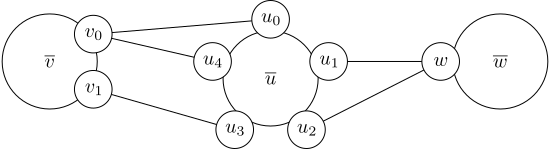
\includegraphics[width=\columnwidth]{images/intro-l2-l3}
\caption[Interfaces et voisins]{On distingue soigneusement les {\em interfaces
de $\overline{u}$} ($u_0, \ldots, u_4$), les {\em interfaces voisines de $\overline{u}$} ($v_0,
v_1, w$) et enfin les voisins de $\overline{u}$ ($\overline{v}, \overline{w}$).
Ces trois notions sont naturellement liées mais leur confusion est à l'origine
d'erreurs historiques.}
\label{fig:intro-l2-l3}
\end{figure}

Cela a une importance considérable dans l'interprétation de la sortie de l'outil
\traceroute (\refchap{traceroute}). La confusion entre {\em lien entre
interfaces}, et {\em lien entre noeuds} est la cause d'erreurs
historiques~\cite{willinger,paristraceroute}. Dans tout notre travail, nous
désignerons toujours une {\em interface} par une lettre romaine ($v$) et un {\em
noeud} comme une classe d'interfaces appartenant à ce noeud ($\overline{v}$).
Cette notation se justifie par le fait que les noeuds sont presque
systématiquement désignés implicitement par l'une de leurs interfaces plutôt que
par un nom propre. L'ensemble des interfaces d'un noeud $\overline{v}$ est tout
simplement identifiée à $\overline{v}$, et l'ensemble des voisins d'un noeud
$\overline{v}$ sera noté $V(\overline{v})$. Le problème de déterminer si deux
interfaces $v_0$ et $v_1$ appartiennent à un même noeud $\overline{v}$ est connu
sous le nom d'{\em anti-aliasing}. Le problème inverse, déterminer la liste de
toutes les interfaces d'un noeud donné $\overline{v}$, est un problème ouvert
connu sous le nom d'{\em aliasing}. Ces deux problèmes seront traités en
profondeur dans le~\refchap{udpping}.

Dans ces deux définitions, nous ignorons les interfaces physiques ou logiques
déconnectées d'Internet, par exemple les interfaces connectées à un réseau privé
(par exemple ${\tt 192.168.0.1}$), les boucles locales (${\tt 127.0.0.1}$), ou
toutes les autres interfaces dont l'adresse correspond à une adresse invalide sur Internet
(RFC 5735\rfc{5735}). On note $\IPSet$ l'ensemble des adresses \ip valides sur
Internet.

Lorsqu'un noeud ${\overline v}$ appartient à la fois à $V_2$ et $V_3$, comme
c'est le cas des routeurs et des hôtes, et lorsqu'aucune confusion n'est
possible, on identifiera une interface physique dans \LL et l'adresse \ip de
l'interface correspondante au niveau logique. Lorsqu'un noeud ${\overline v}$
dispose d'une unique interface $v$, et lorsqu'aucune confusion n'est possible,
on identifiera $v$ et ${\overline v}$. C'est fréquemment le cas des hôtes
terminaux ({\em end hosts}) qui ne disposent que d'une seule interface physique
et logique les reliant à Internet.

À l'aide du formalisme que nous avons introduit, nous pouvons définir plus
formellement certains types de noeuds.

\begin{definition}[Switch]
On appelle \switch tout noeud $\overline{v} \in V_2$ qui n'est pas également un
noeud de \LLL ($\overline{v} \notin V_3$).
\label{def:switch}
\end{definition}

\begin{definition}[Hôte]
On appelle {\em hôte} ({\em host}) tout noeud $\overline{v} \in V_2$ qui est
également un noeud \LLL ($\overline{v} \in V_3$).
\label{def:host}
\end{definition}

\begin{definition}[Hôte terminal ({\em end-host})]
On appelle {\em hôte terminal} tout {\em hôte} qui possède une unique interface.
\label{def:endhost}
\end{definition}

\begin{definition}[Routeur] On appelle {\em routeur} tout {\em hôte} qui n'est
pas un {\em hôte terminal}.
\label{def:routeur}
\end{definition}

Comme nous l'avons déjà mentionné, même si ces appellations ne correspondent pas
toujours à l'appellation commerciale, en termes de topologie physique ou
logique, on peut toujours s'y ramener, et c'est pour cette raison que nous avons
choisi de conserver un formalisme justifié par des considérations topologiques
plutôt que commerciales. Par exemple, ce que l'on appelle commercialement un
{\em hub} est équivalent à un \switch selon la définition qui précède. Ce que
l'on appelle commercialement un {\em switch \LLL} est équivalent à un routeur
selon la définition qui précède. De même, les "routeurs" domestiques que l'on
peut trouver chez des particuliers sont le plus souvent configurés en mode
passerelle ({\em gateway}) et selon notre définition ils sont équivalents à
des hôtes terminaux, puisqu'ils ont une unique interface connectée à Internet.
La topologie physique est donc formée exclusivement de {\em switches}, de {\em
routeurs} et d'{\em hôtes terminaux} ({\em end-hosts}), et la topologie logique
est formée exclusivement de {\em routeurs} et d'{\em hôtes terminaux}.

Nous pouvons alors définir et distinguer les {\em chemins} et les {\em routes}
sur Internet.

\begin{definition}[Chemin sur Internet] On appelle {\em chemin} sur $G_2$ (\resp
sur $G_3$) une suite $({\overline v_0}, \ldots, {\overline v_n})$ de {\em
noeuds} de $V_2$ (\resp de $V_3$) tels que $({\overline v_i}, {\overline
v_{i+1}}) \in E_2$ (\resp $\in E_3$).
\label{def:chemin}
\end{definition}

\begin{definition}[Route sur Internet] On appelle {\em route} sur $G_2$ (\resp
sur $G_3$) une suite $((v_0', v_1), \ldots, (v_n', v_{n+1}))$ telle que $v_i$ et
$v_i'$ sont des interfaces d'un certain noeud ${\overline v_i}$ de $V_2$ (\resp
de $V_3$) , et $v_i'$ est une interface capable de communiquer avec l'interface
$v_{i+1}$ au niveau \LL (\resp~\LLL).
On appelle {\em chemin sous-jacent} de cette route le chemin $({\overline v_0},
\ldots, {\overline v_{n+1}})$, et {\em trace} de cette route la suite des {\em
interfaces entrantes} $(v_1, \ldots, v_n)$.
\label{def:route}
\end{definition}

La distinction entre {\em chemin} et {\em route} est importante, mêmes si les
deux notions sont très proches. À toute route correspond un chemin sous-jacent,
mais la notion de route est plus précise, car elle décrit la liste des
interfaces entrantes et sortantes parcourures par des paquets \ip. Un chemin, en
revanche, ne décrit qu'une suite de n\oe{}uds empruntés et abstrait
l'information concernant les interfaces parcourues. Un chemin est donc une
information moins précise qu'une route.

Les deux topologies d'Internet les plus couramment étudiées sont très liées, car
les noeuds de la topologie physique sont également des noeuds de la topologie
logique, et les liens de la topologie logique sont induits par la topologie
physique. L'inverse n'est pas vrai: deux noeuds connectés dans la topologie
logique ne sont pas nécessairement connectés dans la topologie physique
(\reffig{intro-l2-l3-topo}).

\realfig{intro-l2-l3-topo.png}{Topologie physique et topologie logique
d'Internet} {Un ensemble d'entités connectées à Internet dans la topologie
physique (à gauche), et leur projection dans la topologie logique (à droite).
Les hôtes (cercles) sont tous connectés à un switch (carré). Ce type de
configuration physique se projette en une clique dans la topologie logique.}
{intro-l2-l3-topo}

La distinction entre ces deux topologies est très importante. Conceptuellement,
elles représentent des objets différents et leurs caractéristiques ne sont pas
directement équivalentes. On peut par exemple imaginer une topologie logique
avec un degré moyen très élevé correspondant à une topologie physique avec un
degré moyen très faible. Sur la \reffig{intro-l2-l3-topo}, on constate par
exemple que pour un même réseau, la topologie logique est de degré moyen
$N/(N+1)$, alors que la topologie logique est de degré moyen $(N+1)/2$. Du point
de vue de la mesure, ce sont également des topologies très différentes puisque
les primitives de mesure que nous décrirons, telles que \traceroute ou \ping,
exploitent des caractéristiques spécifiques des couches \LL ou \LLL. Enfin,
certains phénomènes tels que le {\em tunneling}\rfc{1853} n'ont pas de sens au
niveau physique puisqu'ils interviennent uniquement au niveau logique. Nous
verrons que les méthodes de mesure que nous avons étudié exploitent le plus
souvent les relations entre les deux topologies pour déduire des informations
sur l'une ou l'autre.


\section{Approches historiques}

Dans cette section, nous positionnerons la problématique historique dans
laquelle s'inscrit cette thèse. Nous verrons d'abord à quels questionnements
historiques elle s'attache à contribuer (\refsubsec{intro-genesis}), l'approche
historique de modélisation pour y répondre (\refsubsec{intro-models}), et les
approches historiques de cartographie pour les compléter
(\refsubsec{intro-maps}).

\subsection{Génèse de la problématique}
\label{subsec:intro-genesis}

La lecture la plus communément admise de son histoire fait d'Internet l'héritier
d'un certain nombre de réseaux de commutation de paquets, son ancêtre le plus
direct d'un point de vue architectural étant {\em ARPANET}. Le premier lien de
ce réseau est bien identifié, et il reliait entre elles les universités de
Californie, Los Angeles (UCLA) et l'institut de recherche de Stanford. Ce lien a
été établi le 29 octobre 1969. Le 5 décembre de la même année, 2 noeuds
supplémentaires furent connectés: l'univeristé de l'Utah et l'université de
Californie, Santa Barbara. En 1972, le réseau comportait 23 sites, et cinq ans
plus tard, en 1977, plus d'une centaine d'ordinateurs étaient connectés.
Jusqu'à cette année-là, la société {\em BBN Technologies}, travaillant sur le
projet {\em ARPANET}, parvenait à conserver une carte précise et
vraissemblablement exacte de tous les noeuds et liens du réseau
(\reffig{bbn-maps-early}, \cite{bbn-report}).
Mais dès lors, ses rapports deviennent plus précautionneux, et suggèrent déjà
que la carte pourrait s'avérer inexacte, ne reflétant que des informations
déclaratives (\reffig{bbn-maps-1977}).

\begin{figure}[!ht]
\centering
\subfloat[1969]{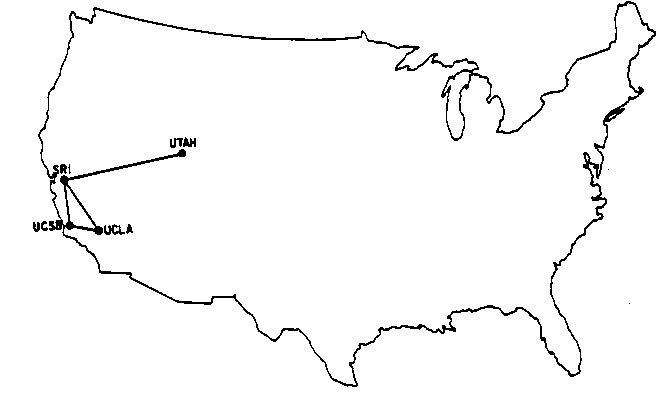
\includegraphics[width=0.5\columnwidth]{images/arpa-1969}}
\subfloat[1971]{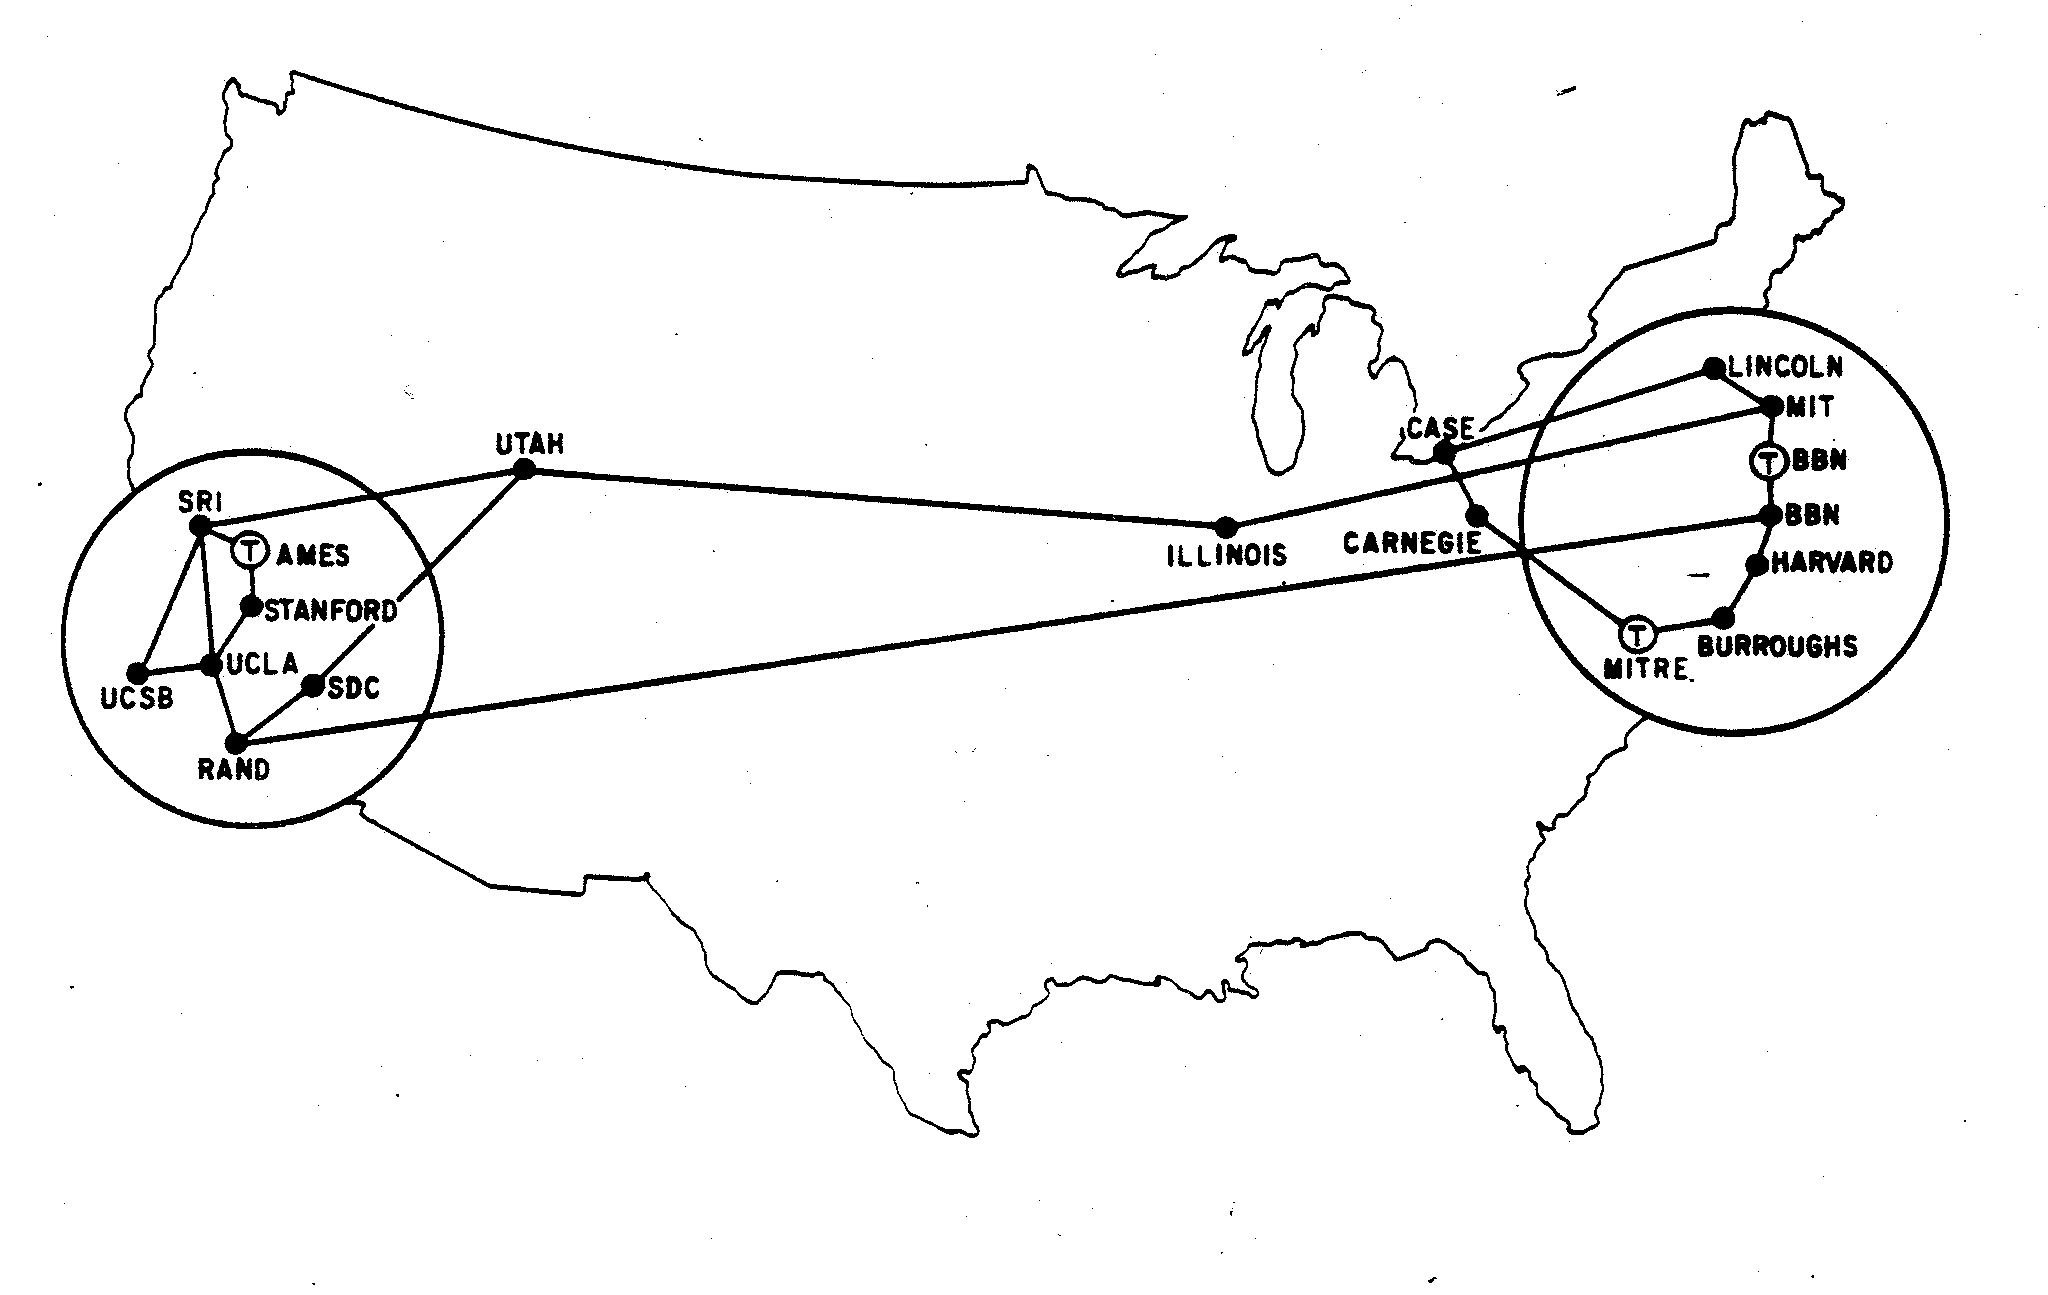
\includegraphics[width=0.5\columnwidth]{images/arpa-1971}} \\
\subfloat[1973]{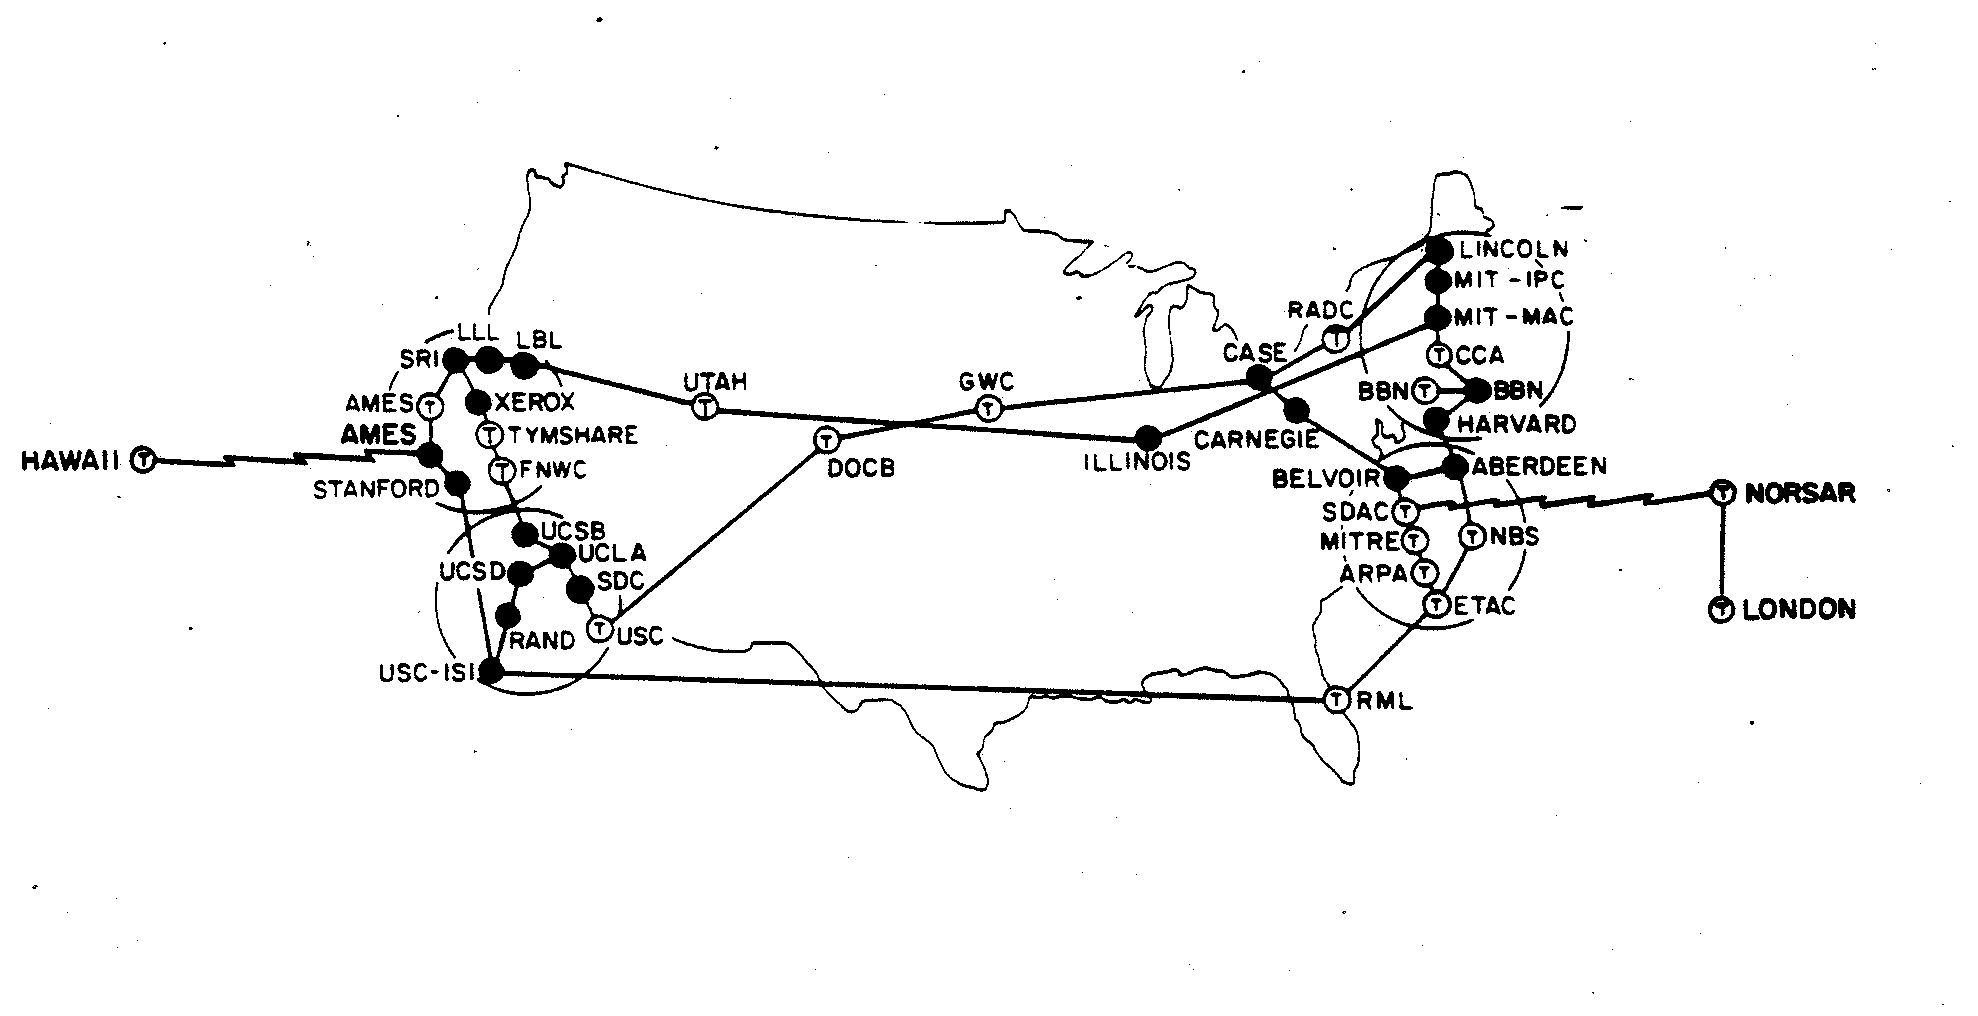
\includegraphics[width=0.5\columnwidth]{images/arpa-1973}}
\subfloat[1974]{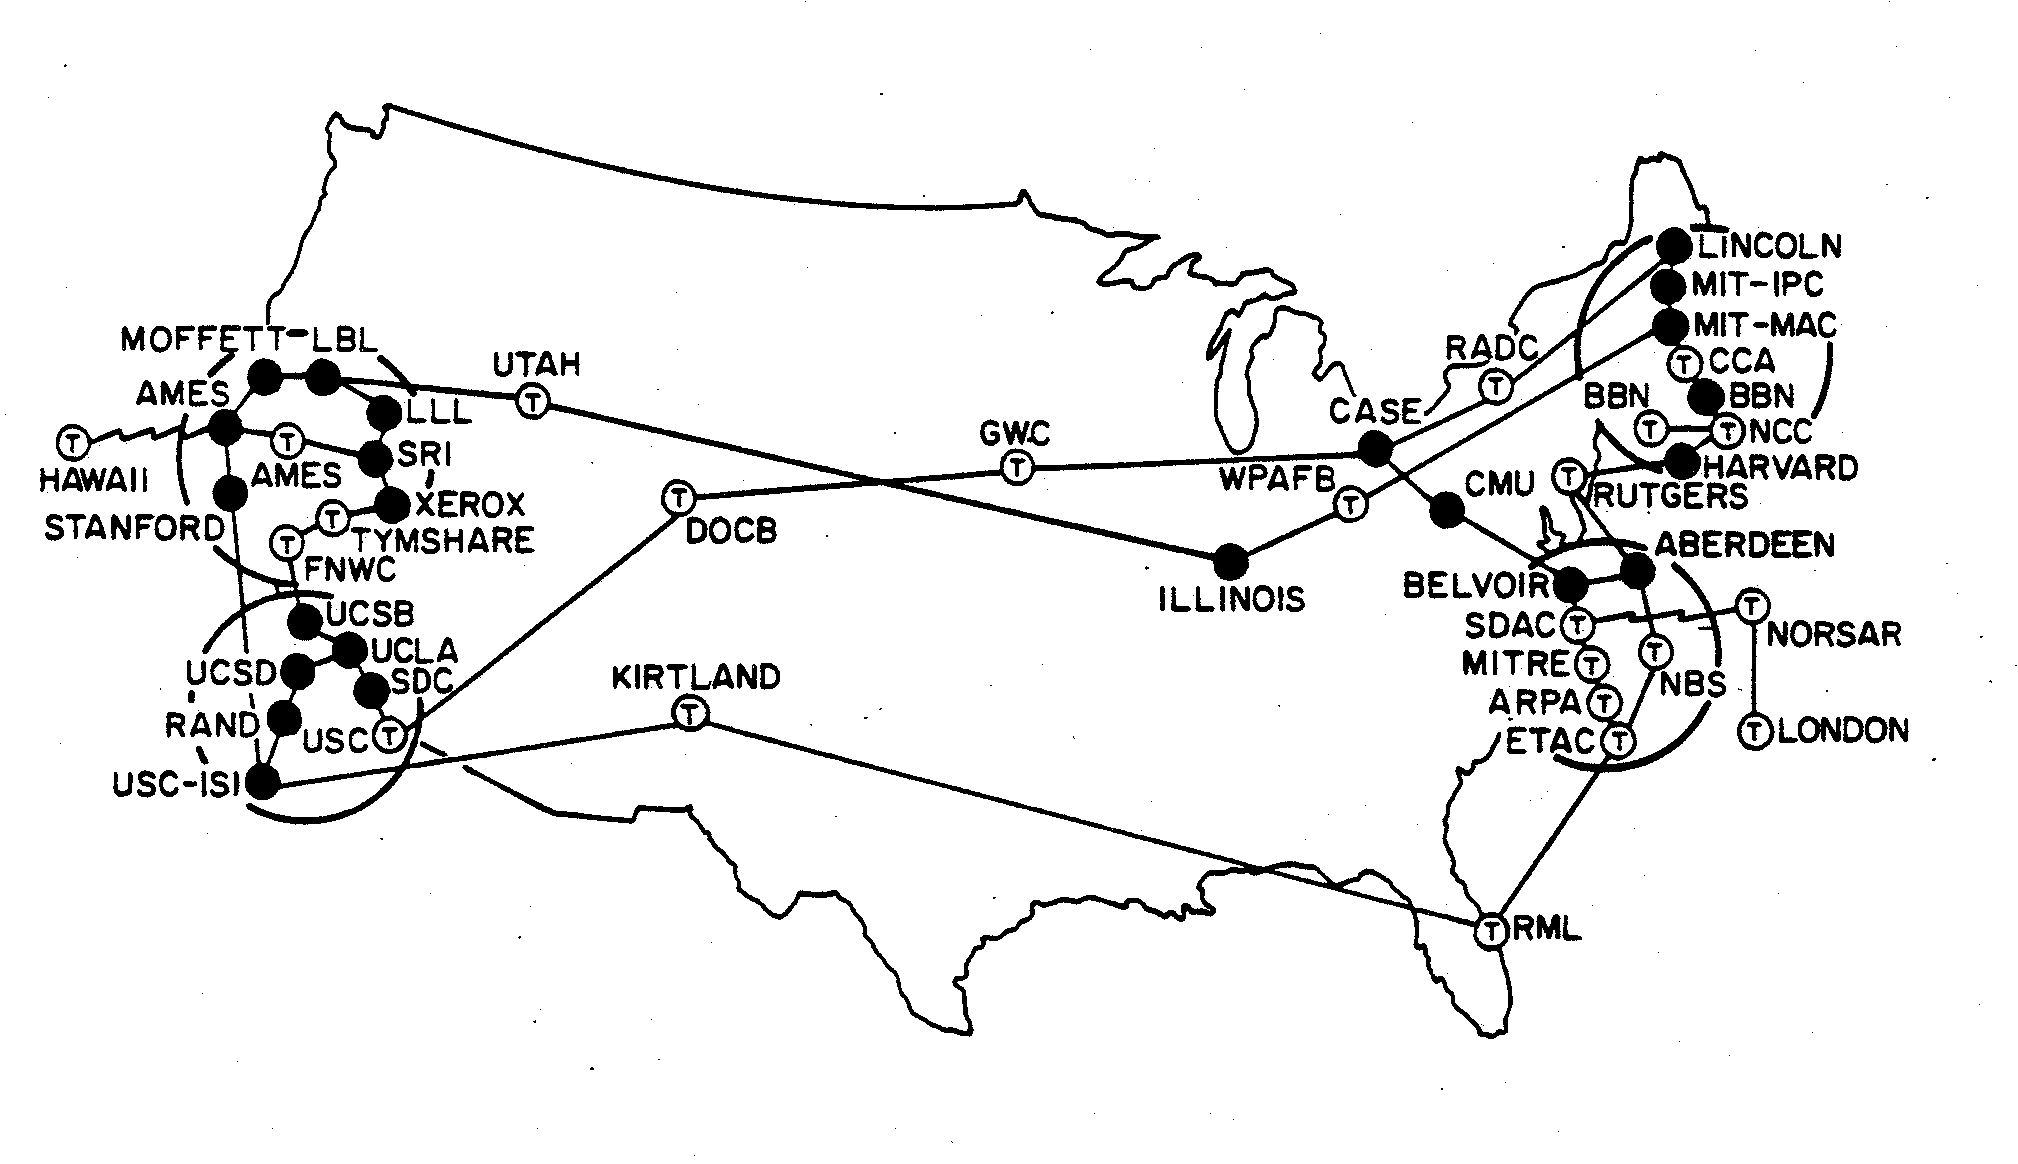
\includegraphics[width=0.5\columnwidth]{images/arpa-1974}} \\
\subfloat[1976]{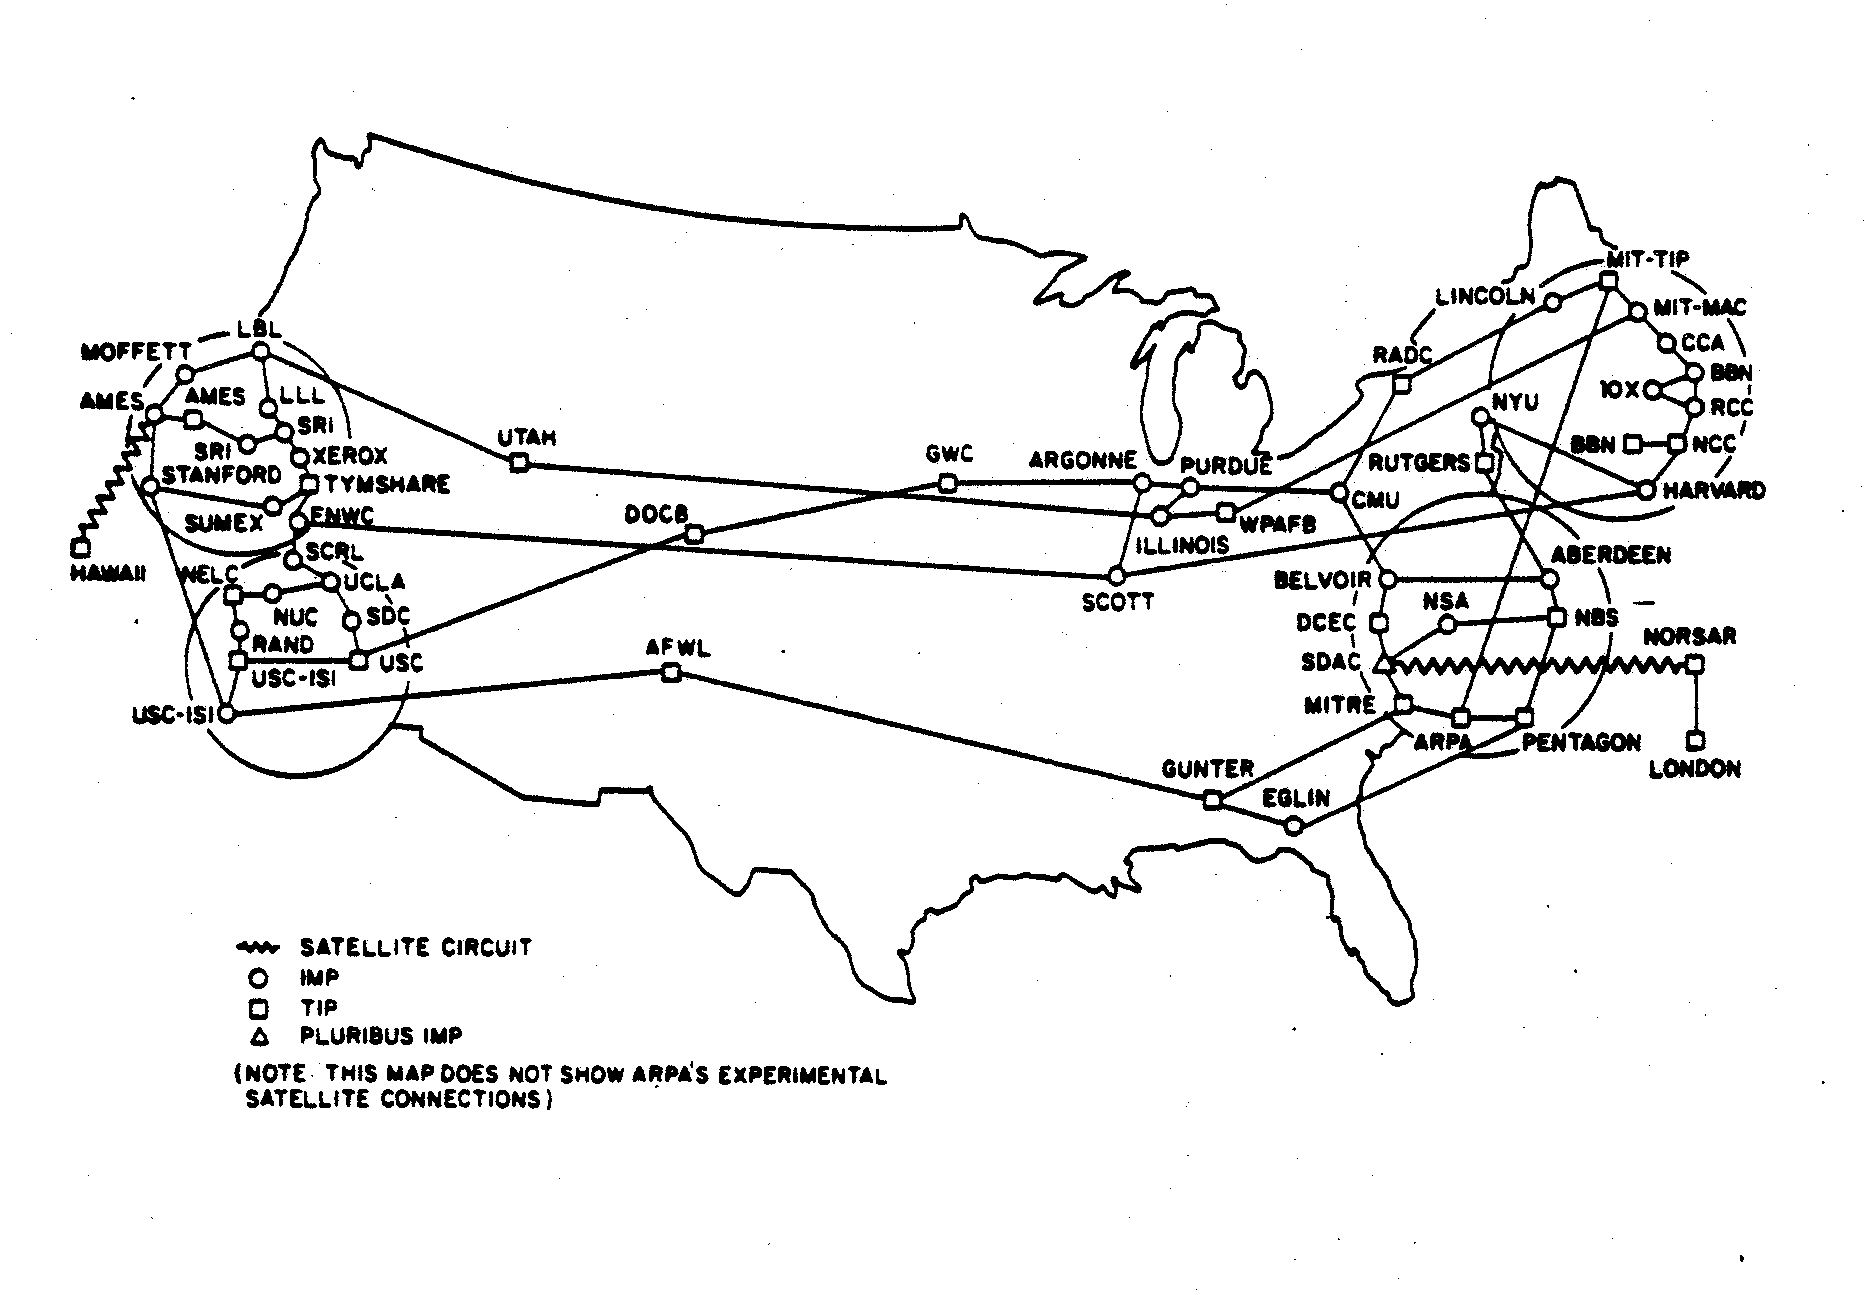
\includegraphics[width=0.5\columnwidth]{images/arpa-1976}}
\subfloat[1977]{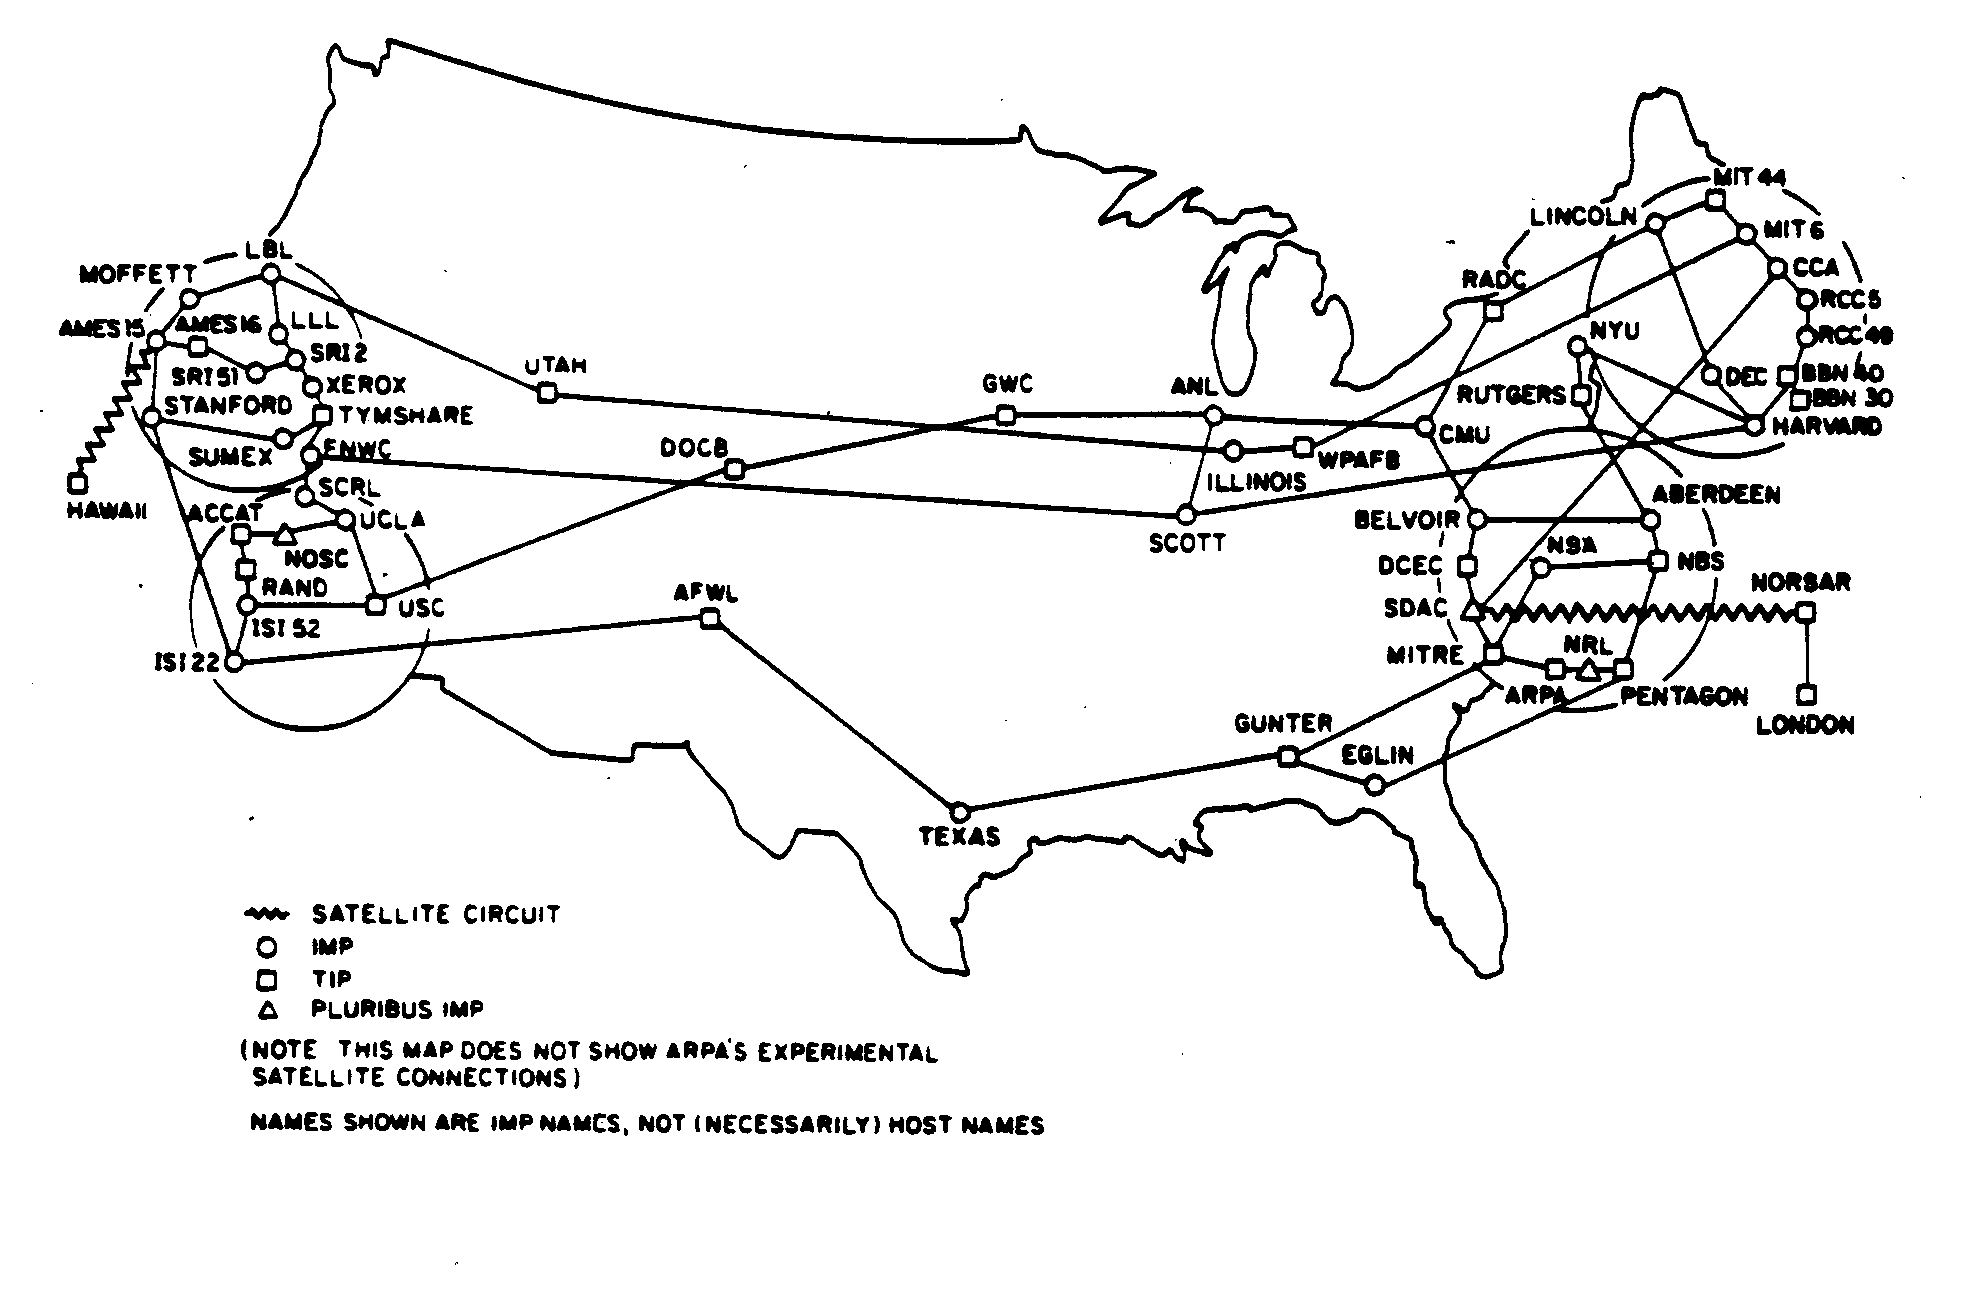
\includegraphics[width=0.5\columnwidth]{images/arpa-1977}} 
\caption{Cartes du réseau {\em ARPANET}, 1969-1977\cite{bbn-report}}
\label{fig:bbn-maps-early}
\end{figure}

\begin{figure}[!ht]
\centering
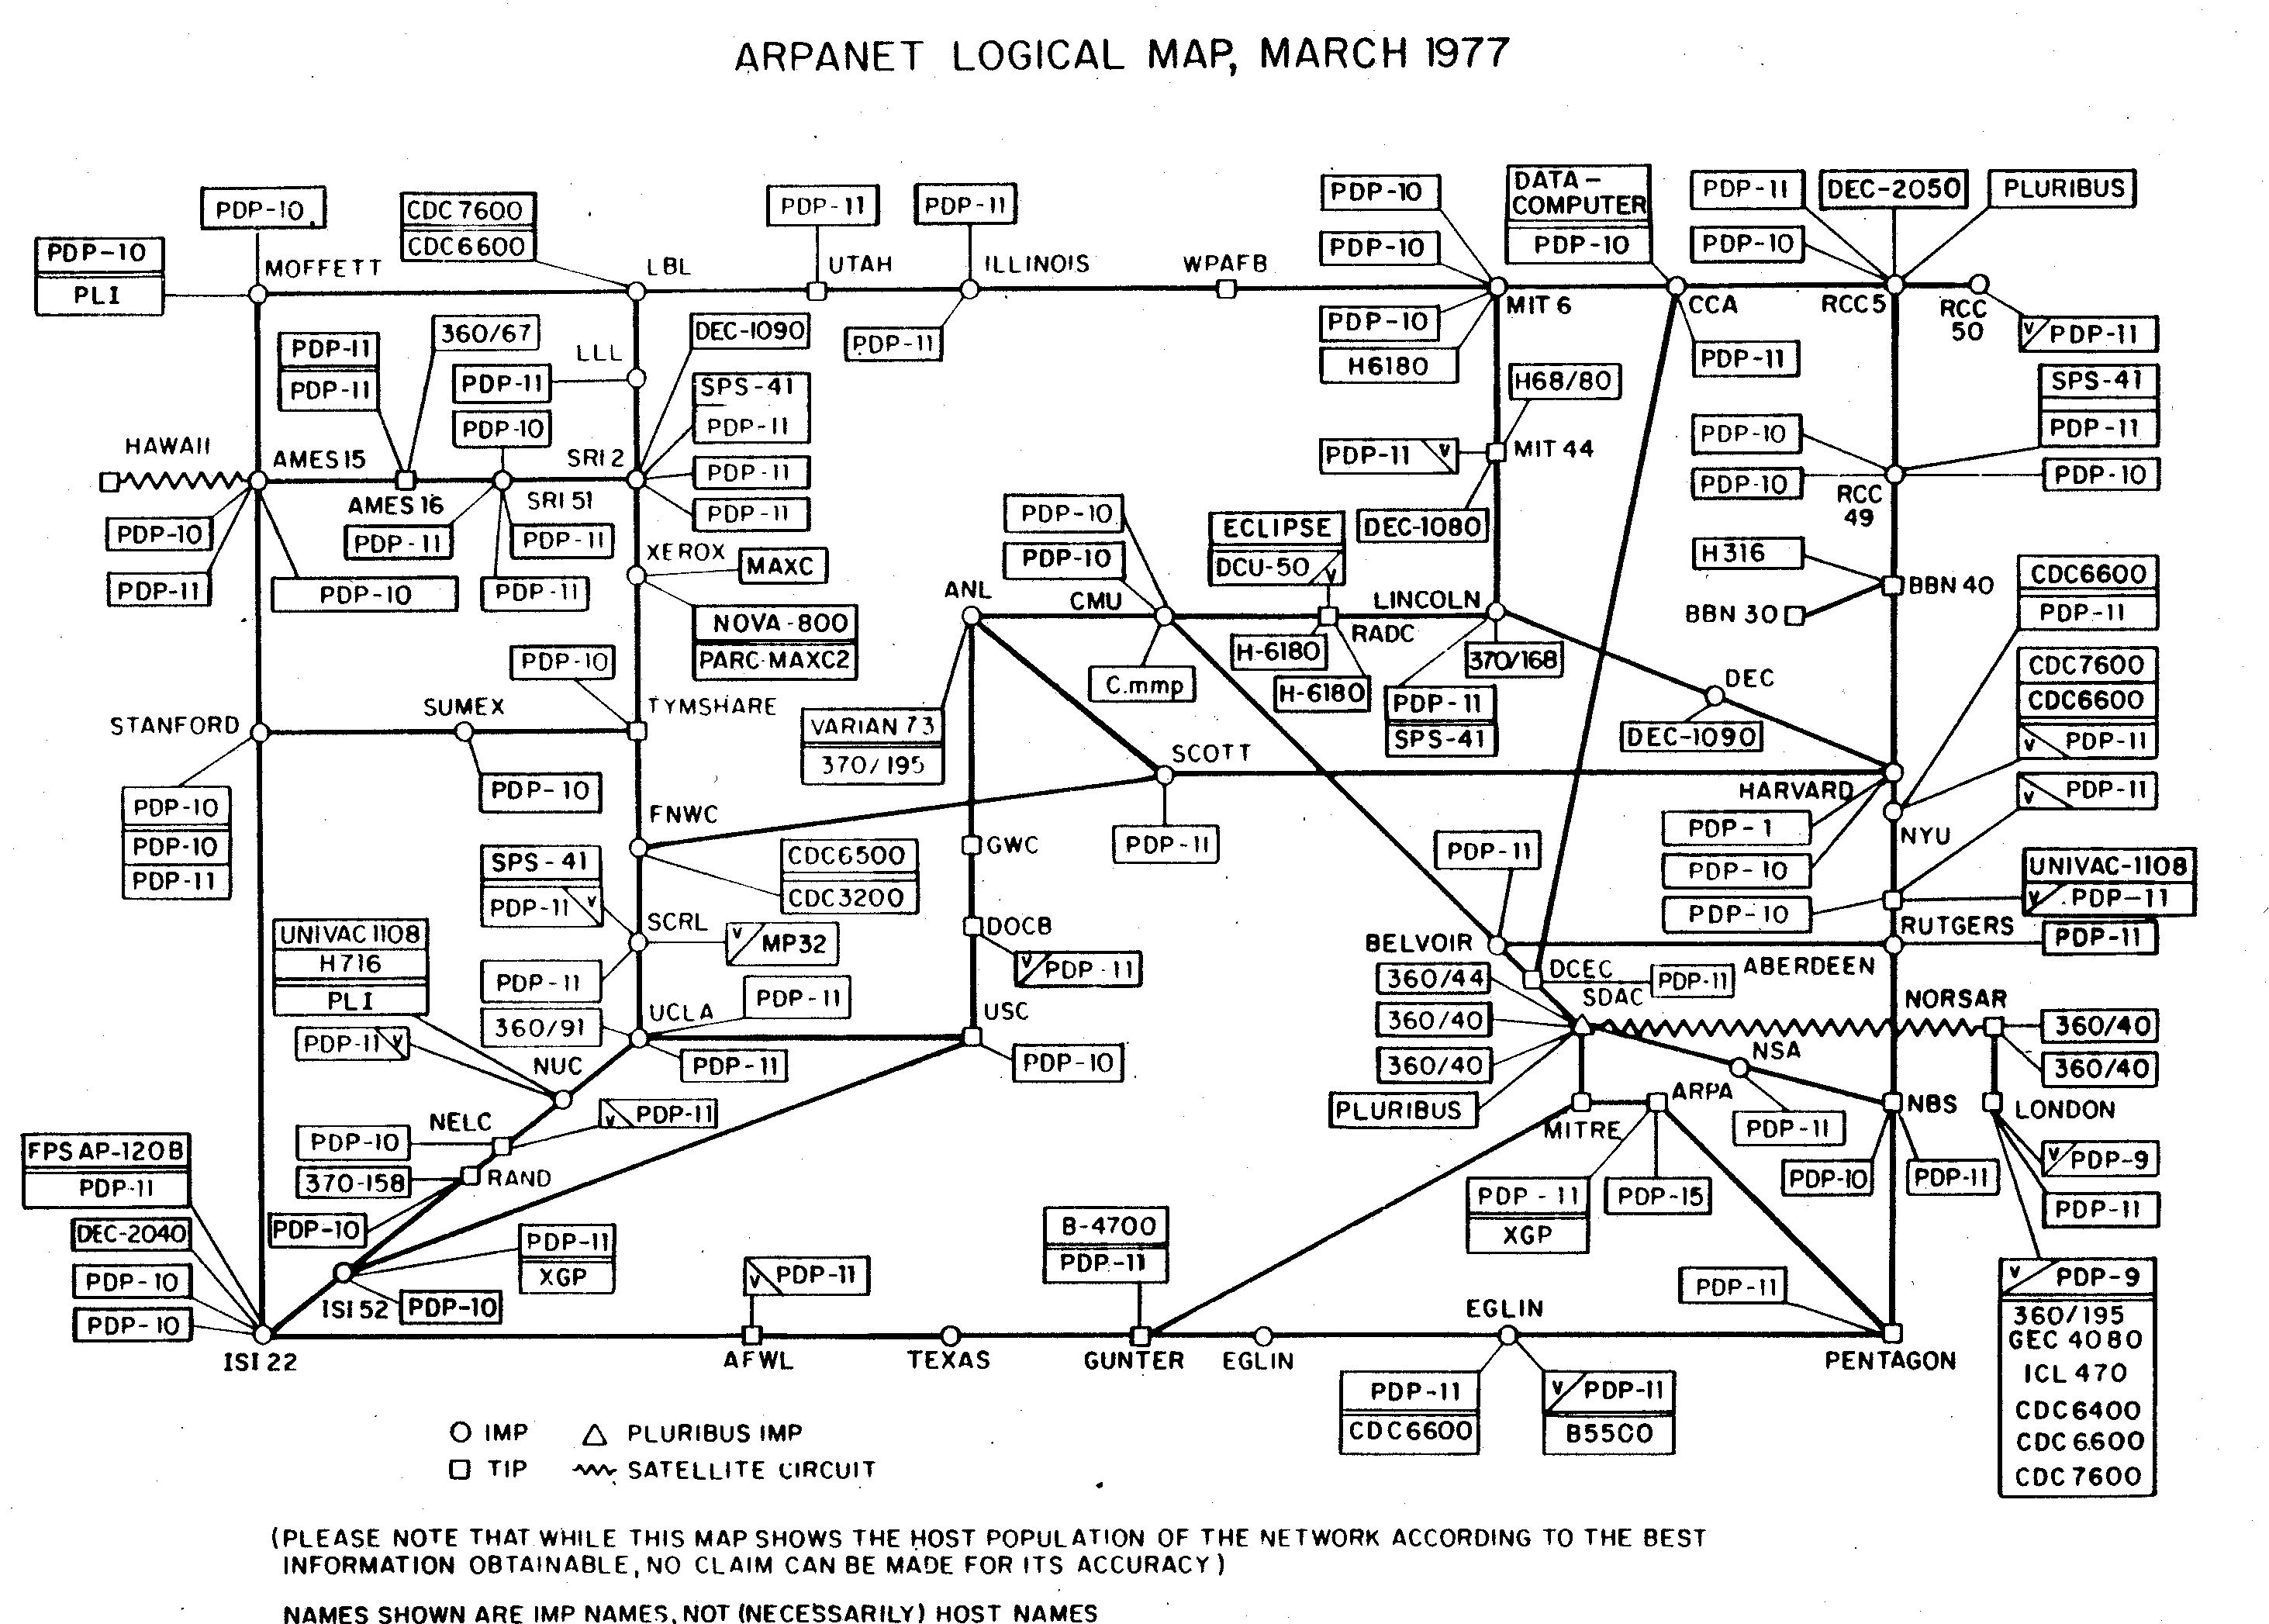
\includegraphics[width=\columnwidth]{images/arpa-1977-approx}
\caption{Carte {\em best effort} du réseau {\em ARPANET}, 1977\cite{bbn-report}}
\label{fig:bbn-maps-1977}
\end{figure}

Cette incertitude va naturellement augmenter avec l'explosion de la taille du
réseau et l'adoption de \tcp/\ip au début des années 80, permettant de connecter
entre eux plusieurs sous-réseaux. La structure de ces sous-réseaux n'est plus gérée de manière
centralisée, et {\em BBN} abandonne l'idée de la connaître; elle ne se contente
déjà plus que d'éditer une carte basée sur des informations déclaratives à
l'échelle inter-réseaux (\reffig{bbn-maps-1985}).

\begin{figure}[!ht]
\centering
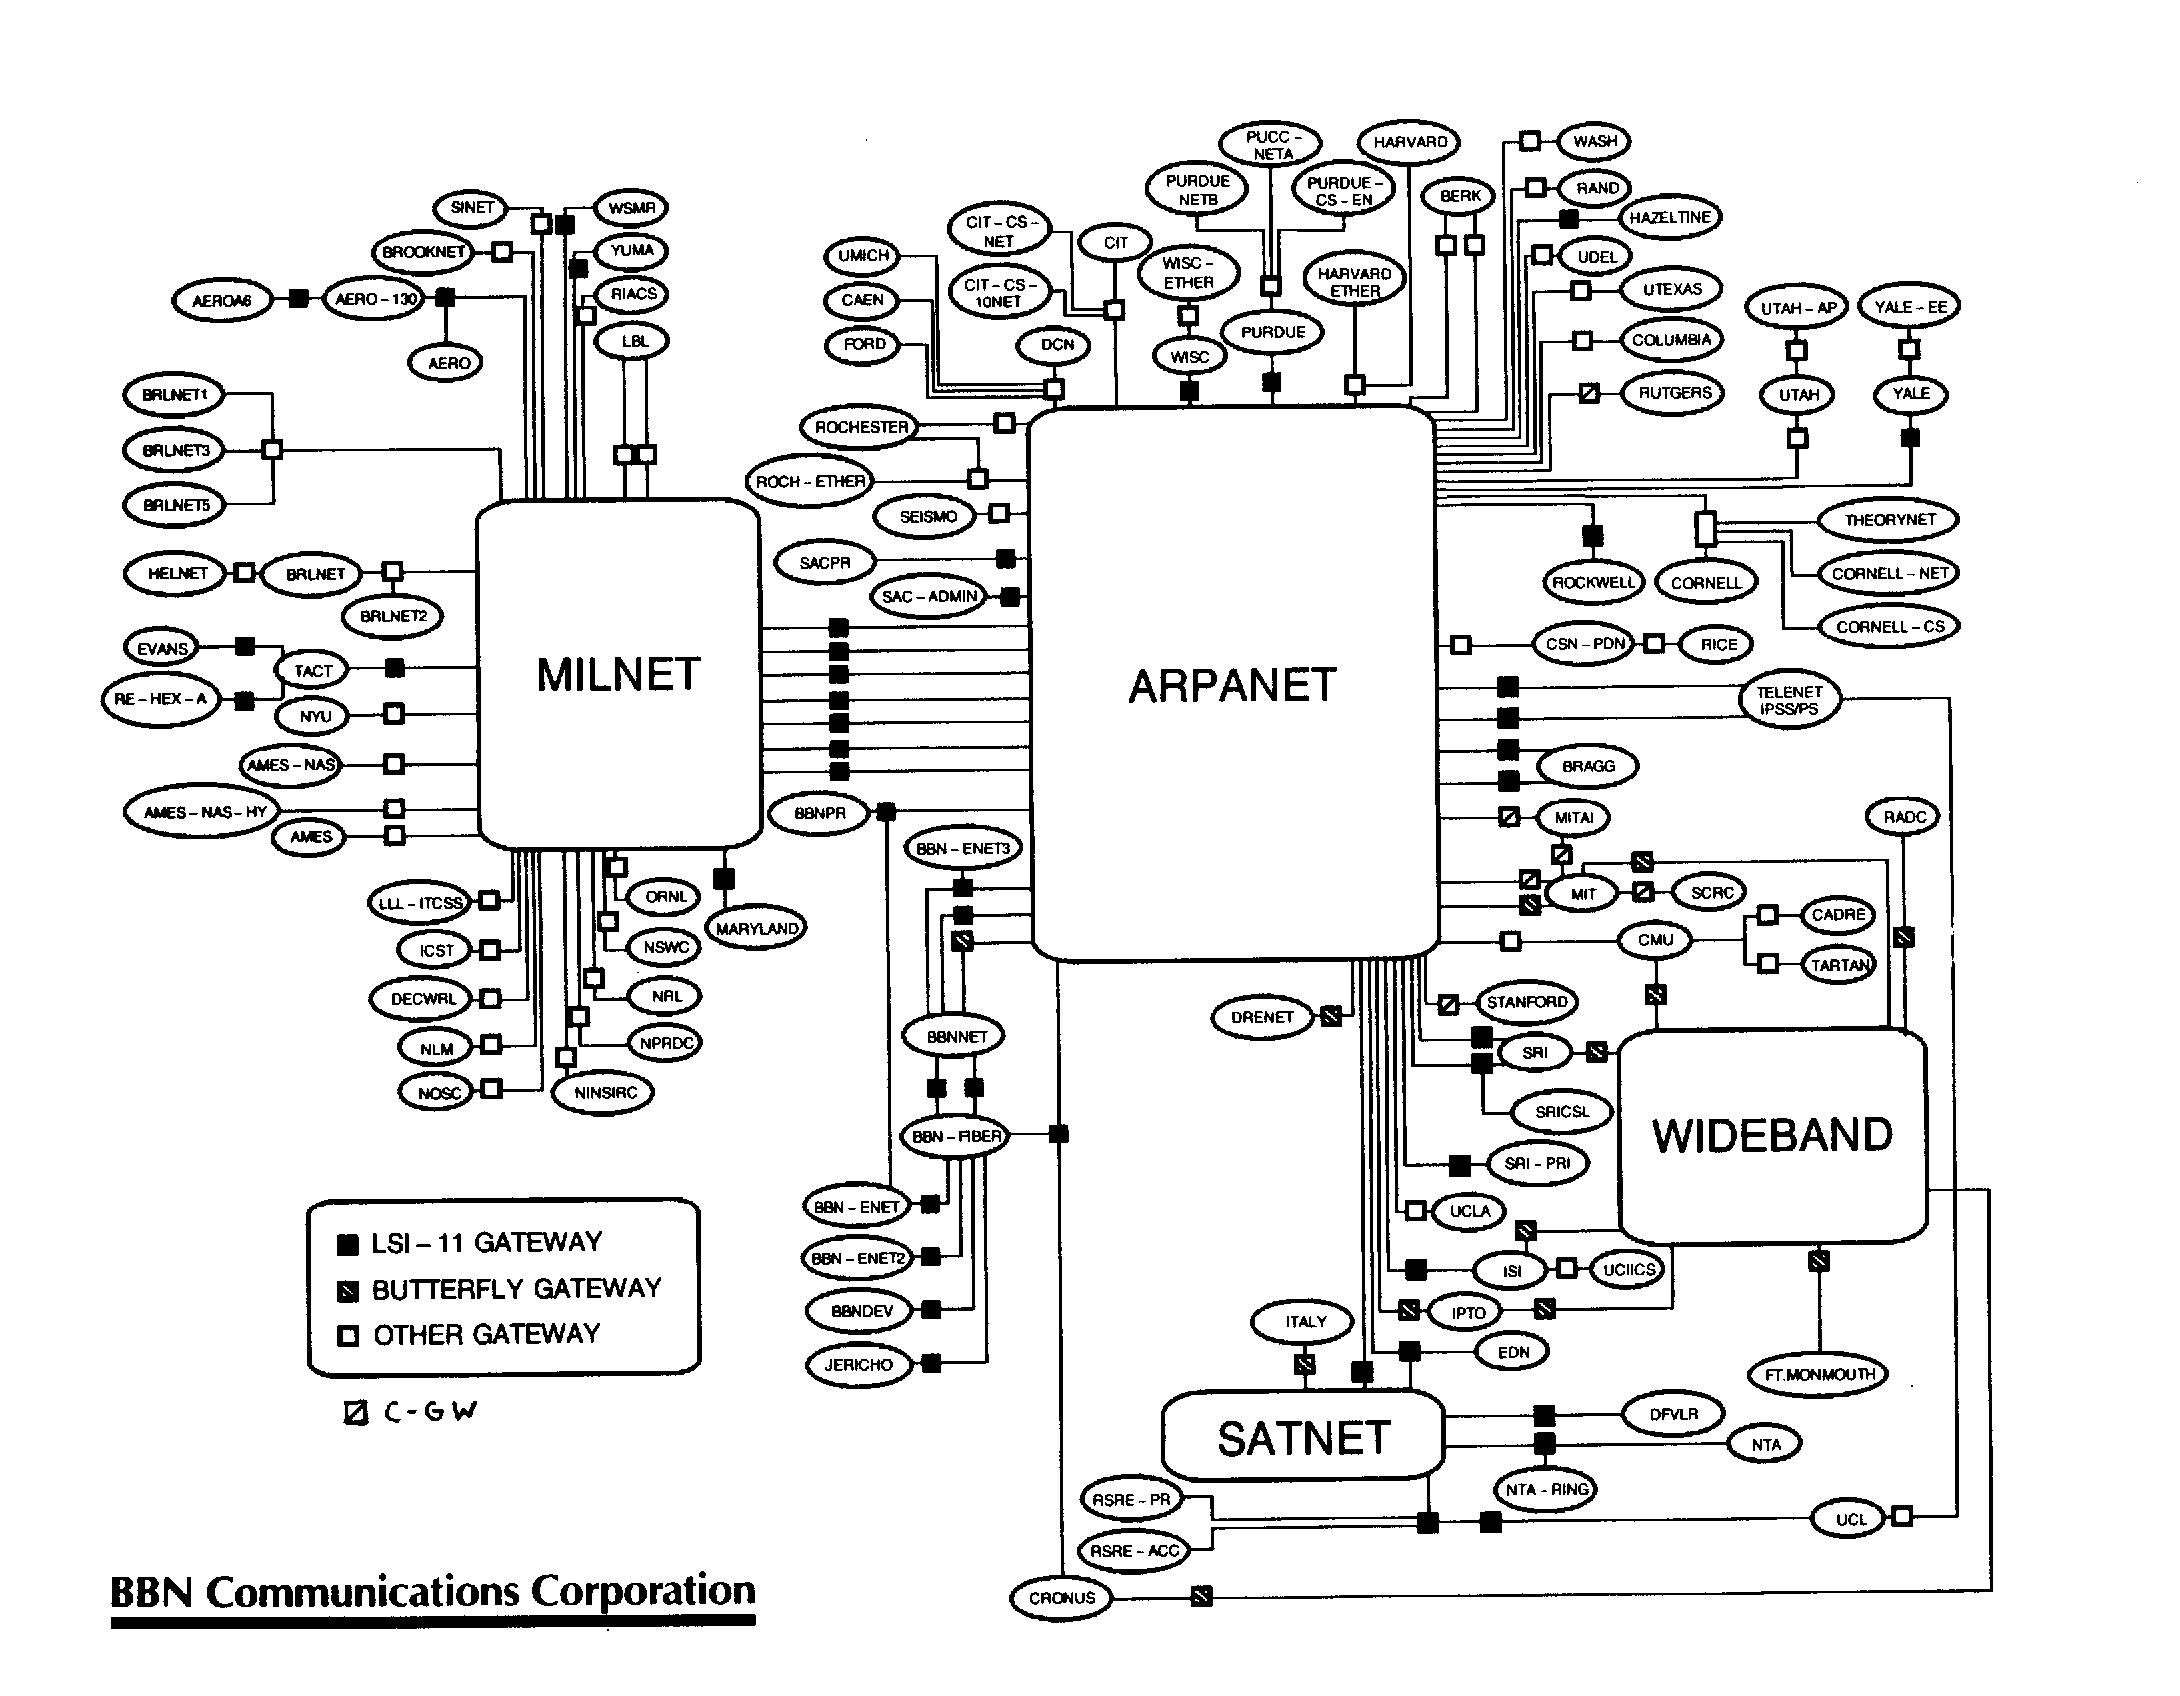
\includegraphics[width=\columnwidth]{images/inet-1985}
\caption{Carte {\em best effort} du réseau \tcp/\ip, 1985\cite{bbn-report}}
\label{fig:bbn-maps-1985}
\end{figure}

À la fin des années 80, l'inter-réseau \tcp/\ip prend le nom d'{\em Internet}.
Au début des années 90, l'accès est ouvert au grand public, et le nombre
d'ordinateurs connectés dépasse les 10 millions. Le seuil des 100 millions est
franchi au début des années 2000; au début des années 2010, le nombre
d'ordinateurs connectés dépasse le milliard. 
(\reffig{inet-hosts-growth}, \cite{isc-report})


\begin{figure}[!ht]
\centering
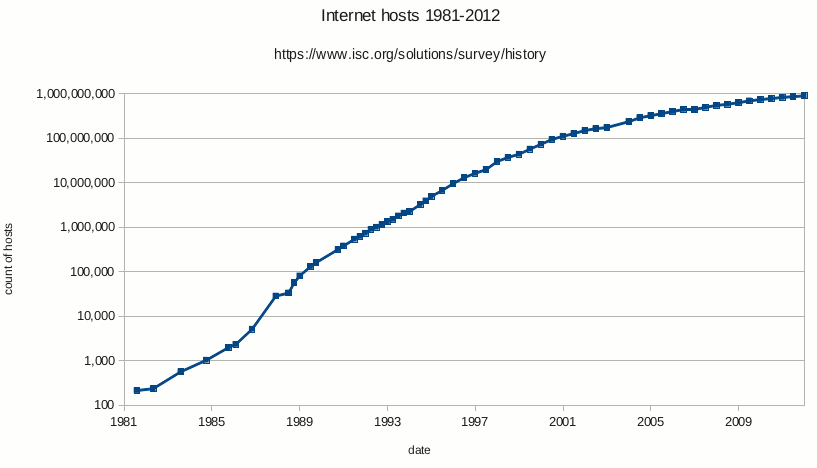
\includegraphics[width=\columnwidth]{images/inet-hosts-growth}
\caption{Croissance du nombre d'hôtes connectés au réseau,
1981-2012\cite{isc-report}}
\label{fig:inet-hosts-growth}
\end{figure}


Avec l'importence qu'a prise Internet aujourd'hui, l'utilisation d'un {\em
modèle} d'Internet est extrêmement fréquente. Pour analyser le réseau, prédire
son comportement, ou tout simplement le décrire, on a besoin d'une
représentation aussi réaliste que possible vis à vis des caractéristiques
auxquelles on s'intéresse. C'est particulièrement important lorsqu'on traite du
réseau directement, comme par exemple pour traiter du routage ou de la
robustesse des télécommunications, mais également lorsqu'on s'intéresse à des
abstractions au dessus du réseau, comme par exemple le Web ou l'économie
numérique.

\subsection{Modèles formels d'Internet}
\label{subsec:intro-models}

À cause de la très grande taille d'Internet et surtout, de sa gérance très
décentralisée, par sa nature même d'inter-réseaux, l'espoir de maintenir une
carte exacte du réseau au fur et à mesure de sa construction a depuis longtemps
été abandonné. Une des premières approches historiques, dite approche {\em
montante}\footnote{De l'anglais {\em bottom-up}} repose sur une idée simple:
le réseau est certes complexe, mais il ne serait qu'une combinaison logique de
composantes simples résultant de l'ingénierie humaine. Il faudrait donc
correctement représenter ces composantes simples, et combiner ces
représentations, pour obtenir une représentation fidèle du réseau. Cette
approche est celle qui correspond à la vision pédagogique d'Internet, et elle
est issue de la communauté des réseaux. Elle considère le réseau avant tout
comme une création d'ingénierie, et non comme un objet
d'observation. Une conséquence directe de cette vision est qu'avec les bonnes
prémisses, on devrait pouvoir représenter fidèlement le réseau. En pratique,
cette approche conduit à la conception d'{\em algorithmes de génération de
graphes} supposés représenter fidèlement Internet.

Le modèle historique le plus populaire est celui de Waxman
\etal\cite{waxman1988routing} et repose sur des graphes aléatoires contraints
par la distance euclidienne entre les noeuds. Ce modèle est efficace pour
représenter de petits réseaux de l'échelle d'{\em ARPANET}. Des modèles plus
détaillés\cite{doar1996better,zegura1997quantitative} ont été établis par la
suite, en combinant plusieurs modèles selon des variétés de sous-graphes locales
correspondant à différentes échelles administratives du réseau.

Hélas, en plus de la complexité réelle des composantes et leur variété en dépit
d'efforts de standardisation, la combinaison extrêmement complexe de ces
composantes repose sur des paramètres topologiques, correspondant précisément à
l'implémentation des autorités locales decentralisées. Ces paramètres sont le
plus souvent laissés à l'intuition du modélisateur, ce qui conditionne le
réalisme de la représentation.\cite{paxson1997we}

\subsection{Cartographie d'Internet}
\label{subsec:intro-maps}

Face à la dépendance des approches {\em montantes} de modélisation à des
paramètres topologiques inconnus, une idée nouvelle a émergé à la fin des années
90 et au début des années 2000. Cette approche, dite {\em descendante}, consiste
à considérer le réseau comme un objet d'observation, au même titre que peuvent
l'être des objets non synthétiques tels que la faune ou la flore. Il s'agit
alors de {\em mesurer} le réseau afin d'en établir une {\em carte}, et
d'utiliser cette carte pour déterminer les propriétés topologiques du réseau,
qu'on injecterait ensuite dans les modèles formels.

L'étude de Govindan \etal\cite{govindan1997analysis} (1997) s'attache à la
cartographie de la topologie inter-domaines, c'est à dire la topologie au niveau
\as, et repose sur les traces \bgp, qui sont utilisées pour extraire la
distribution de degré et le diamètre de cette topologie. Les travaux de Pansiot
et Grad\cite{pansiot1998routes} (1998) se focalisent pour la première fois sur
le réseau au niveau des hôtes \LLL, plus précisément aux routeurs, en utilisant
des sondes \traceroute paramétrées avec l'option LSRR ({\em Loose Source and
Record Route}). Ces derniers travaux ont initié un large ensemble de recherches
pour plus d'une décennie sur la cartographie du réseau, qui adoptent tous une
stratégie similaire, décomposant les travaux en une partie de cartographie du
réseau reposant sur des observables, et une partie sur l'extraction de
propriétés topologiques à partir de ces cartes. Le travail ayant eu la plus
forte influence à cet égard est vraisemblablement celui de
Faloutsos\etal\cite{faloutsos1999power} (1999), qui estime que le réseau
s'organise en distribution de degré en loi de puissance.

Beaucoup de travaux ont suivi reposant sur des mesures \traceroute,
\tracetree\cite{sarac2004tracetree,latapy2008radar}, \mrinfo\cite{merlin} et
d'autres outils analogues, ainsi que des regards critiques sur la fiabilité de
telles mesures. Ces critiques portent d'abord sur la fiabilité technique des
outils, par exemple face à la dynamique ou aux mesures d'obfuscation pratiquées
par les administrateurs réseaux (blocage de trafic \icmp, non-respect des
directives de {\em source-routing} et {\em route-recording}\ldots)
\cite{GunesS09,paristraceroute,keys2010internet,keysiffinder,roughan201110,pansiot2012,alias-bias}.
Mais au delà des problèmes techniques, peut-être résolubles, de ces méthodes,
une critique plus fondamentale apparaît :
les cartes construites à partir de ces mesures seraient intrinsèquement biaisées
\cite{roughan201110,willinger,LakhinaBCX03,AchlioptasCKM09,DallAstaABVV06,GuillaumeL05,GuillaumeLM06,latapy2008complex,MDBP10},
dans la direction de topologies en loi de puissance. En effet, il apparaît
qu'observer le réseau en aggrégeant les traces de routes issues d'un nombre
limité de n\oe{}uds en confère une vision formée d'une réunion d'arbres, ce qui
biaise les degrés observés.

Pour tenter de remédier à ce biais, des efforts importants ont été réalisés pour
augmenter la taille et la qualité des cartes, mais ces améliorations se sont
avérées insuffisantes à éliminer le
biais\cite{willinger,latapy2008complex,BarfordBBC01}. La nature même des
réunions d'arbres depuis un nombre limité de racines biaise la topologie, et
augmenter la taille de ces arbres ne résoud pas ce biais.

\section{Notre approche}
\label{subsec:intro-POM}

Après plus d'une décennie de recherches, le bilan de la cartographie d'Internet
est mitigé. L'idée d'utiliser des outils de diagnostic réseau pour {\em
observer} le réseau comme un objet naturel est une contribution indéniable qui a
permis d'améliorer sa compréhension, mais les espoirs de déterminer les
paramètres de modélisation permettant de représenter fidèlement le réseau au
niveau macroscopique n'ont pas été satisfaits. Notre lecture est qu'à l'origine,
l'objectif de la cartographie était bien de déterminer ces paramètres, mais
qu'elle est progressivement devenue un objectif propre, qui l'a d'une certaine
manière cantonnée dans une classe de problèmes qui a été mise en évidence comme
intrinsèquement biaisée.

Pour cette raison, nous avons choisi de développer une approche différente.
Plutôt que d'utiliser des outils de mesure pour établir des cartes sur
lesquelles ont pourrait {\em lire} les propriétés topologiques qui nous
intéressent pour les injecter dans des modèles, {\bf nous utilisons ces outils
de mesure pour mesurer {\em directement} ces propriétés topologiques}, plutôt
que de faire appel à une carte intermédiaire.
Nous espérons, de cette manière, éviter le biais intrinsèque de la {\em
cartographie}, qui tend à donner une vision du réseau comme une réunion d'arbres
correspondant à l'observation du réseau depuis un nombre limité de points de
vue.

Notre démarche repose sur une compréhension claire de nos objectifs et une
maîtrise de chacune des étapes de notre démarche. Notre objectif est
d'obtenir une évaluation très fiable d'une propriété topologique du réseau et
pour l'obtenir, nous devons maîtriser les biais potentiels induits par les
mesures empiriques. Nous nous proposons de mettre en place la démarche théorique
suivante, pour mesurer des propriétés topologiques du réseau.

\begin{itemize}
  \item Soit une propriété du réseau définie par la distribution d'une
  certaine fonction $p :
  V \supseteq V' \rightarrow {\mathbb R}$ (propriété de noeuds) ou $p : E
  \supset E' \rightarrow {\mathbb R}$ (propriété d'aretes).
  \item Soit une primitive de mesure $\tilde{p} : V' \supset V'' \rightarrow
  {\mathbb R}$ ou $\tilde{p} : E' \supset E'' \rightarrow {\mathbb R}$, qui
  estime $p$ sur un sous-ensemble des noeuds ou des aretes concernées par $p$,
  c'est à dire telle que $\tilde{p} = p_{|V''}$ ou $\tilde{p} = p_{|E''}$.
  \item Soit une procédure d'échantillonage de $V''$ ou de $E''$ telle que la
  distribution de $p$ sur un échantillon converge vers la distribution de
  $p$ sur $V'$ ou que la distribution de $p$ sur un échantillon converge vers la
  distribution de $p$ sur $E'$.
  \item On tire un échantillon $\tilde{V'}$ ou $\tilde{E'}$ et on mesure
  $\tilde{p}$ sur cet échantillon.
  \item On estime alors que la distribution de $p$ sur $\tilde{V'}$ ou
  $\tilde{E'}$ est égale à la distribution de $\tilde{p}$, et donc que la
  distribution de $p$ sur $V'$ ou $E'$ est égale à la distribution de
  $\tilde{p}$ sur l'échantillon.
\end{itemize}

Cette méthode nous permet d'identifier clairement les potentiels biais, et de
distinguer les biais d'implémentation (calcul de $\tilde{p}$), les biais
topologiques (procédure d'échantillonage), et les biais statistiques
(convergence de la distribution).

\section{Organisation}

Cette thèse présente les travaux que nous avons réalisé pour explorer la
pertinence et la faisabilité de la mesure orientée propriété de la topologie
d'Internet, dans le cas particulier où la propriété d'intérêt est la
distribution de degrés, ou plus exactement les distributions de degrés des
topologies \LL et \LLL.
Elle suit une organisation générale chronologique, qui correspond à la
progression de nos travaux : nous avons d'abord exploré une approche inspirée
des mesures basées sur \traceroute pour mesurer la distribution de degré de la
topologie logique (\refchap{traceroute}), puis nous avons conçu une primitive de
mesure très fiable et un meilleur protocole d'échantillonage pour mesurer la
distribution de degrés de la topologie physique (\refchap{udpping}), que nous
avons exploré en profondeur en mesurant les tables de routages
(\refchap{revtables}). Chacune de ces sections suit en revanche un découpage
réalisé {\em a posteriori} et qui nous semble amener de la manière la plus
pertinente les conclusions que nous en avons tiré et les perspectives qu'elles
ont ouvertes (\refchap{conclusion}).
